%Began 17 May 2025  
\documentclass[letterpaper,x11names,svgnames,10pt]{article}
\usepackage{amsmath}
\usepackage{hyperref}
% the \hypersetup{keyvals} commented out below is stored in an external hyperref.cfg file
% to enable the pagebackref=true option
%\hypersetup{%dvips, % not needed for  pdflatex
%	pagebackref=true,
%	pdfauthor={Iam The Author},
%	hyperfigures,
%	bookmarks=true,
%	bookmarksnumbered=true,
%	bookmarksopen=true,
%	colorlinks=true, %if true, link borders absent
%	pdfborder={1 1 1},
%	citecolor=blue,
%	linkcolor=blue,
%	urlcolor=blue,
%}
\usepackage{url}
\usepackage{svg}
\usepackage{graphicx}
\usepackage{xcolor}
\usepackage{float}
\usepackage{natbib}

\topmargin -0.50in
\oddsidemargin 0.25in
\textwidth 6.50in
\textheight 9.00in

%%%-------------------------------------------
%%% TO BE EDITED FOR EACH NEW VOLUME GENERATED 
%%%-------------------------------------------
	\def\authorName{I Am The Author}
	\def\authorFirstMidNameInit{I.\ T.\ }
	\def\authorLastName{Author}
	\def\dateGenerated{\today}
	\def\volNumber{I}
	\def\mdgBookTitle{Musical Dice Game \\ \vspace{1.5mm} English Country Dances \volNumber}
	\def\mdgBookSubTitle{Musikalisches W\"{u}rfelspiel, K.Anh.C30.01 (1792/93)}
	\def\theBookSeries{Wonders of the Musical World 1ecd}
	\def\theBookPublisher{Libre Edition Press}
	\def\theBookPublisherLogo{../images/1ed.png}
	\def\theBookFrontCover{../images/FrontCover.pdf}
%%%-------------------------------------------
%%%

\def\uline{\underline}
%\definecolor{orange}{rgb}{1,0.5,0} % RGB
%\definecolor{light-gray}{gray}{0.95} % shades
%\definecolor{orange}{cmyk}{0,0.5,1,0} % CMYK

\newcommand{\HRule}{\rule{\linewidth}{0.5mm}}

\setlength{\parindent}{0pt}

\DeclareGraphicsExtensions{.pdf,.png}

\setcitestyle{authoryear,round,comma,aysep={,},yysep={,},notesep={, }}

\title{\textsc{\mdgBookTitle}}
\author{\textsc{\authorFirstMidNameInit \authorLastName}}
\date{\textsc{\dateGenerated}}
% -----

\begin{document}

% Book Cover
% File name: mdgBooSVGecdv1-cover.tex
% Purpose: Book Cover
% Instruction: Should be \input{.} just after \begin{document}
{
\topmargin 0.00in
\oddsidemargin 0.45in
\textwidth 8.50in
\textheight 11.50in
\thispagestyle{empty}

\begin{titlepage}

\begin{picture}(0,0)%
\linethickness{67.00pt}
\color{blue!22!black}
\put(-105,85){\line(1,0){6477}}
\put(-105,-612){\includegraphics[clip=true,trim=0.00in 0.45in 0.25in 1.95in, height=11.5in,width=8.80in,keepaspectratio]%
	{\theBookFrontCover}}
\put(-105,-645){\line(1,0){6477}}
\end{picture}

\vspace{-1.50in}

\begin{center}
	\LARGE\textbf{\color{white} \theBookSeries}
\end{center}

\vspace{-0.25in}
\vspace*{2.\baselineskip}
\begin{center} \Huge\textbf{\color{DarkRed!40!Crimson}\em \mdgBookTitle}
\end{center}

\begin{center}
	\Large\textbf{\color{DarkRed!40!Crimson}\em \mdgBookSubTitle}
\end{center}

\begin{center}
	\LARGE\textbf{\color{DarkRed!20!Crimson}\em compiled by \authorFirstMidNameInit \authorLastName}
\end{center}

\vfill
\begin{center}
	\LARGE\textbf{\color{white}\em \theBookPublisher \\ \vspace{-0.25in}}
\end{center}
\end{titlepage}
}




\newpage
% Title Page

${}_{}$\\
\vspace{1.00in}	
\thispagestyle{empty}
\begin{center}
	\HRule \\[0.4cm]
	{\huge \bfseries \mdgBookTitle} \\[0.25cm]
	{\large based on {\em \mdgBookSubTitle} }\\[0.25cm]
	\HRule \\[1.5cm]
	% Author and supervisor
	\begin{minipage}{0.4\textwidth}
		\begin{flushleft} \large
			\emph{Author:}\\
			\authorFirstMidNameInit \textsc{\authorLastName}
		\end{flushleft}
	\end{minipage}
	\begin{minipage}{0.4\textwidth}
		\begin{flushright} \large
			\emph{Supervisor:} \\
			Dr. Communio \textsc{Sanctorum}
		\end{flushright}
	\end{minipage}
	\vfill
	% Bottom of the page
	{\textsc{\Large \theBookSeries}}  \\[0.2cm] 
	\includegraphics*[width=0.15\linewidth]{\theBookPublisherLogo}\\ 
	{\large \theBookPublisher \\
       \dateGenerated }\\
	\vspace{2.50in}
\end{center}
\newpage

%\maketitle		% uncomment if no Front Cover

\tableofcontents\label{tabofcon}

%\extrafloats{182}

\newpage
\section[Introduction]{Introduction\footnote{The information contained in the introduction were culled from the following online resources:
	\citet{wiki_mw2017}, \citet{wam92}, \citet{kv2024}, 
	\url{https://opus-infinity.org/}, and 
	\href{https://www.sciencenews.org/article/mozarts-melody-machine-0}{Mozart's Melody Machine} \citep*{peterson2001}
	}
}
	\begin{center}
	\begin{minipage}{0.4\textwidth}
	\begin{flushleft}
		\begin{center}
			``ANLEITUNG\\
			Englische Contret\"{a}nze mit zwei\\
			W\"{u}rfeln zu componiren, so\\
			viele man will, ohne\\
			etwas von der Musik\\
			oder Composition\\
			zu verstehen."\\
		\end{center}
	\end{flushleft}
	\end{minipage}
	\begin{minipage}{0.4\textwidth}
	\begin{flushright}
		\begin{center}
		``INSTRUCTION\\
		To compose \\
		without the least \\ 
		knowledge of Music \\ 
		so much English Country Dances \\
		as one pleases, by throwing a \\
		certain Number with two Dice."
	\end{center}
	\end{flushright}
	\end{minipage}
	\end{center}

Thus run the German title and English translation of {\it Musikalisches W\"{u}rfelspiel K.Anh.C.30.01 - Englische Contret\"{a}nze (1792/93)}, the Musical Dice Game (MDG) that is closely related to {\it Musikalisches W\"{u}rfelspiel K.\ 516f (1787)}, this latter MDG being the most well-known of MDGs.  Rightly and interestingly so, as the Instructions provided in {\it Englische Contret\"{a}nze} (the manner by which we are going to refer to this MDG from here onward) allow a non-professional musician to generate (``compose") as nearly as 1.4 quadrillions of MDG English Country Dances (ECD).  More precisely, $11^{13}\times 10 \times 2\times 2 = 1\!,380\!,908\!,485\!,757\!,240$; see explanation in Subsection ~\ref{tableFind}.\\  

A {\it Musikalisches W\"{u}rfelspiel} (German for ``musical dice game" or MDG) is a system for randomly ``generating" (e.g., by using a die or two dice) musical compositions from precomposed options and was quite popular throughout Western Europe in the 18th century.  The earliest known MDG is Johann Philipp Kirnberger's {\em Der allezeit fertige Polonoisen und Menuettencomponist (1st ed.\ 1757; rev.\ 2nd ed.\ 1783)} (translated from German as ``The Ever-Ready Polonaise and Minuet Composer").  Other well-known composers that are known to have composed a MDG are C.P.E.\ Bach ({\em Einfall, einen doppelten Contrapunct in der Octave von sechs Tacten zu machen, ohne die Regeln davon zu wissen (1758)}; translated from German as ``A method for making six bars of double counterpoint at the octave without knowing the rules") and Abb\'{e} Maximillian Stadler ({\em Table pour composer des Minuets et des Trios \`{a} la infinie; avec deux dez \`{a} jouer (1780)}; translated from French as ``A table for composing minuets and trios to infinity, by playing with two dice"). \\

{\it Musikalisches W\"{u}rfelspiel K.\ 516f (1787)} was first published by J.J. Hummel in 1793 in Berlin, and was republished in 1796 by Nikolaus Simrock in Bonn (as {\it K.Anh.C.30.01} or {\it K.\ 294d}).  Simrock attributed this work to Wolfgang Amadeus Mozart.  It may have been based on Mozart's manuscript {\it K.Anh. 294d/516f}, written in 1787, consisting of numerous two-bar fragments of music, that appear to be some kind of game or system for constructing music out of two-bar fragments, but contains neither instructions nor hints as to the use of dice.  An \href{(http://www.asahi-net.or.jp/\~rb5h-ngc/e/k516f.htm}{online article} by Hideo Noguchi offers a possible explanation for this attribution. With the release of \href{https://kv.mozarteum.at/en}{\it K\"{o}chel-Verzeichnis 9th ed.\ (2024)}, the {\it KV} index for these works now include {\it K.$^1$deest, K.$^1$Anh.C 30.01/294d, K.$^3$Anh.\ 294d, K.$^6$516f} and \href{https://kv.mozarteum.at/en/work/musikalisches-alphabet-6025}{\it K.$^9$Anh.H 24.11}. \\

This book is a collection of 250 Musical Dice Games (MDG) ECDs generated according to the rules given in {\it Englische Contret\"{a}nze}.  The scores of the generated ECDs, which were initially written using the \texttt{abc} environment of Chris Walshaw, were converted to Scalar Vector Graphics (SVG) images and were then pre-processed with Inkscape to be included in \LaTeX\ to produce this book.


\section{\em K.Anh.C30.01 - Englische Contret\"{a}nze}

\subsection{Rules}\label{genRules}

The Rules provided in {\em Englische Contret\"{a}nze} generate MDG ECDs consisting of 16 measures.  The first eight (8) measures are played then repeated, with a variation on the 8th measure on the repeat leading to the 9th measure.  The last eight measures are then similarly played with the 16th measure remaining the same even on the repeat. \\

The following Rules are followed for generating each ECD:
\begin{enumerate}
	\item [1.] For each measure from the first to the 16th, two dice are tossed and the sum of the two faces that come up is obtained.  Hence, 16 two-dice tosses (with possible outcomes from the set \{2, 3, 4, 5, 6, 7, 8, 9, 10, 11, 12\}), one two-dice toss for each measure, are needed to generate an ECD.   
	\item [2.] Table~\ref{fig:0tab1} is then used to determine which measure number from the Table of Measures (Figures~\ref{fig:meas1} to \ref{fig:meas4}) is to be used for obtaining the notes for the particular measure of the ECD corresponding to the outcome of the two-dice toss.  The possible outcomes of a two-dice toss (2 to 12) are given (stub items) on the left-hand side of Table~\ref{fig:0tab1}, while the measure numbers of the ECD-to-be-generated are given at the top of that table (captions or column  headings).
	\item [3.]  For example, suppose for measure 1, the outcome of the two-dice toss is 5.  If we now look for measure number 1 at the top of Table~\ref{fig:0tab1} and for the outcome 5 on the left-hand side of that table, we obtain 36 as the measure number of the Table of Measures (Figures~\ref{fig:meas1} to \ref{fig:meas4}) to be used for obtaining the notes to be played for the first measure of the ECD to be generated; the notes for the G- and F-clefs (in {\it abc} notation) are:  {\tt [V:1] cC/E/ Gc/e/} and {\tt [V:2] C,2C,2}. An outcome of 11 for the two-dice toss for measure nine (9) of the ECD to be constructed leads us to obtain the notes from measure 61 of the Table of Measures giving the notes: {\tt [V:1] dd$^\wedge$fa} and {\tt [V:2] D,/$^\wedge$F,/A,/F,/ D,C,}.
\end{enumerate}   


\subsection{Table for finding Measure Number from Table of Measures}\label{tableFind}
The table given here (Table~\ref{fig:0tab1}) combines the two tables given on page 2 of {\it K.Anh.C.30.01 - Englische Contret\"{a}nze}, but the contents are exactly as given there.  The leftmost column contains the possible two-dice outcomes, while the topmost row contains the measure number for the MDG ECD to be generated.

\begin{table}[H]
	\centering
	\begin{tabular}{c}
		\centering
		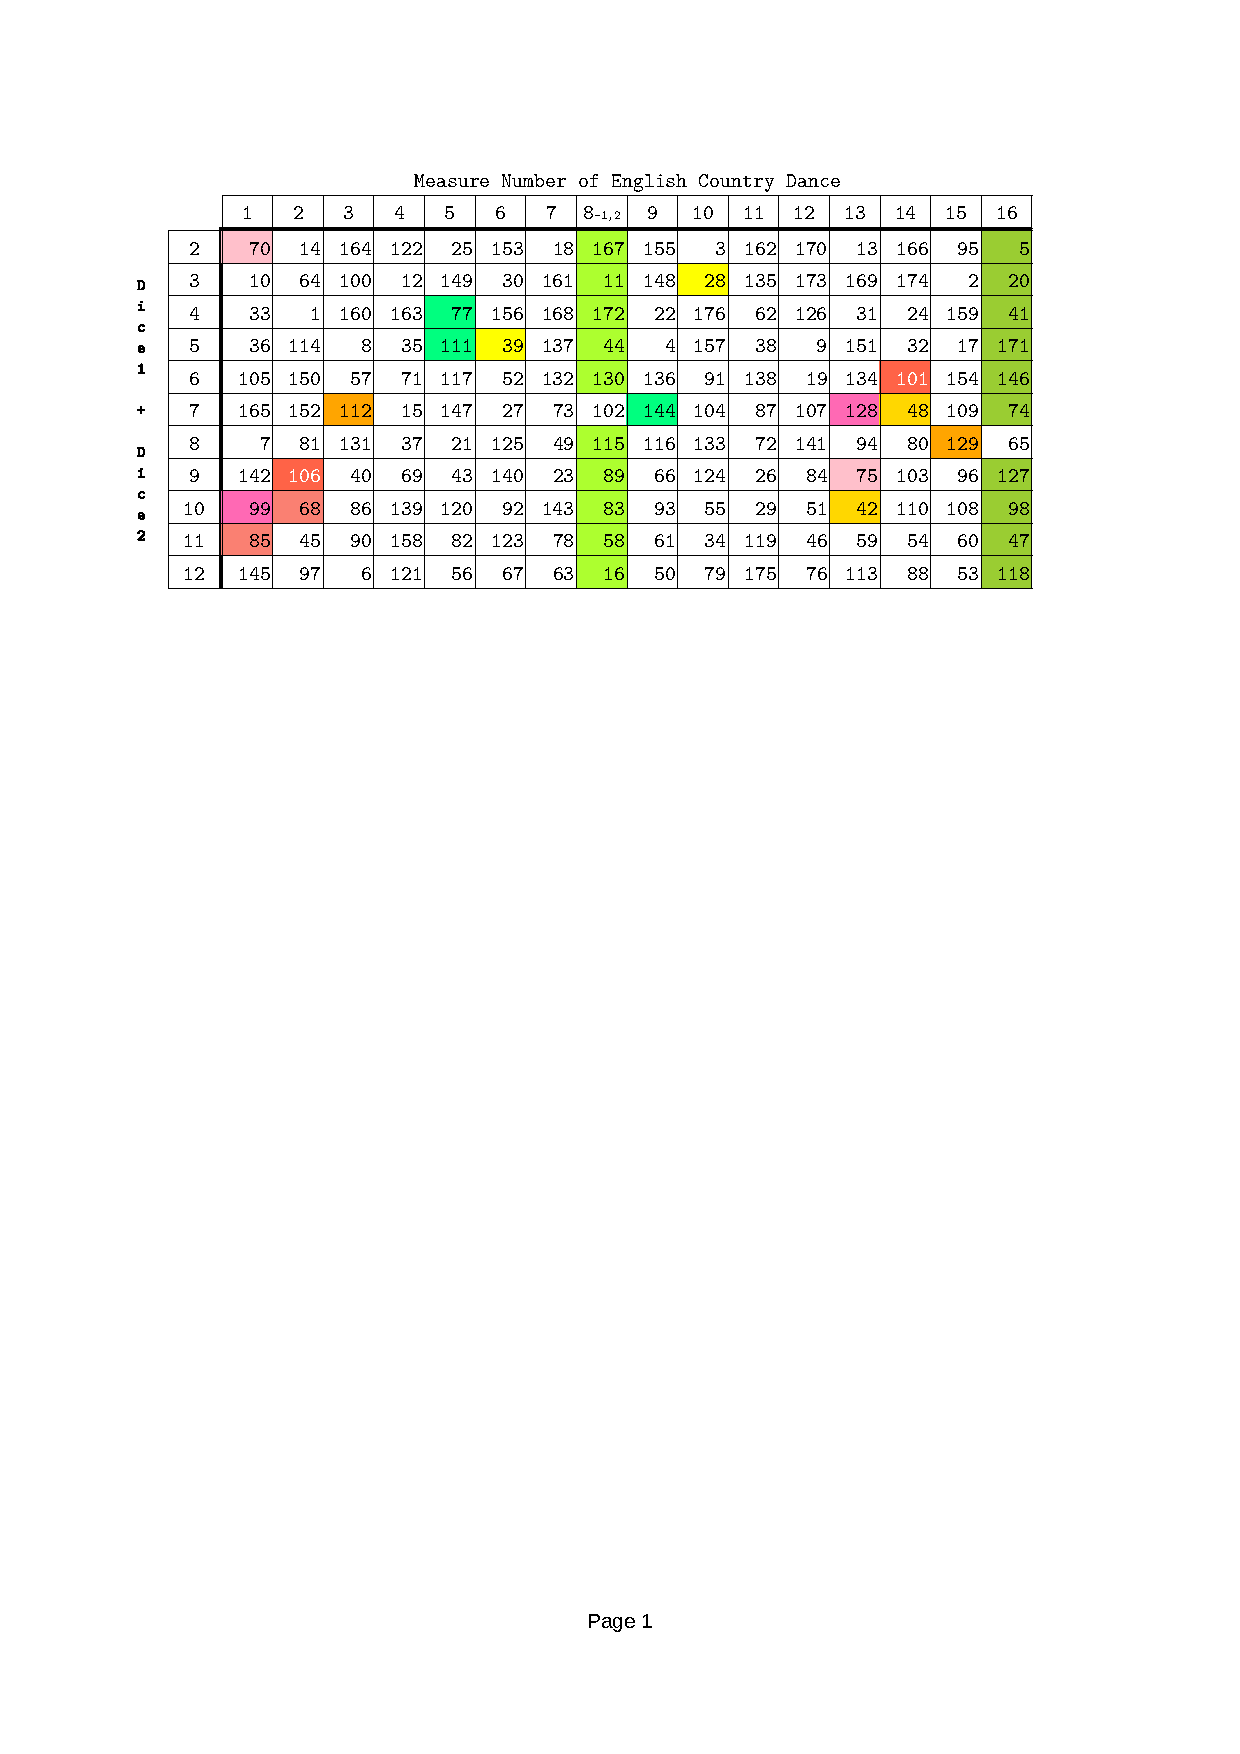
\includegraphics[clip=true,trim=0.90in 7.75in 1.25in 1.00in,scale=0.90]{0TAB1ECc}
	\end{tabular}
	\caption{Measure number to be looked up in the Table of Measures (see Figures~\ref{fig:meas1}, \ref{fig:meas2}, \ref{fig:meas3}, and \ref{fig:meas4}) corresponding to each two-dice outcome per measure of the ECD. Same cell color indicates identical measures. (Based on information from \href{https://opus-infinity.org/dice_games/mozart_contredanse/tables/}{https://opus-infinity.org}.)}
	\label{fig:0tab1}
\end{table}

Although the body of Table~\ref{fig:0tab1} includes $11*16 = 176$ measure numbers, the Table of Measures (Figures~\ref{fig:meas1} to \ref{fig:meas4}) contains only 149 different measures.  The number drops from 176 to 157 for the following reasons: a) for measures 5, 8, and 16, there are 11 choices (listed below each column) for each of the 16 measures (the captions of the table), giving $11*13=143$ different choices for these 13 measures that each have 11 different options; b) there are only two different choices under measure 8 since all of the options have the same set of notes except for dice outcome 7 (measure 102 in Table~\ref{fig:0tab1} and Figure~\ref{fig:meas2};  also, the first pass is different from the repeat, e.g., measures 11 and 16 in the Table of Measures); c) similarly, as for bar 8, there are also only two different choices for the last measure (measure 16) with only the dice outcome of sum 8 (measure 65 in Table~\ref{fig:0tab1} and Figure~\ref{fig:meas2}) being assigned a different set of notes from the 10 other dice outcomes; and, d) for bar 5, there are only 10 different choices since the notes for dice outcomes 4 and 5 are the same (measure 77 and 111 have notes: {\tt [V:1] D$^\wedge$F/A/ d$^\wedge$f} and {\tt [V:2] D,2D,2}).  Thus, the total number of different measures due to these is reduced to $11\times 13 + 2 + 2 + 10 = 157$. Furthermore, there are other pairs/triplets of measures belonging to different columns that are identical, e.g., dice outcome 7 for bar 9 has the same notes as dice outcomes 4 and 5 for bar 5.  More information on such measures is found in Table~\ref{fig:0tab1}, where cells highlighted with the same color indicate identical measures from Figures~\ref{fig:meas1} to \ref{fig:meas4}. Eventually, the total number of different measures drops further from 157 to 149. \\

All told, the total number of unique ECDs generated by the Rules given in Subsection~\ref{genRules} is: $$ \underbrace{11^{13}}_{\tiny\text{Bars 1-4, 6-7, 9-15}} \times \underbrace{10}_{\tiny\text{Bar 5}} \times \underbrace{2}_{\tiny\text{Bar 8}} \times \underbrace{2}_{\tiny\text{Bar 16}} = 1\!,380\!,908\!,485\!,757\!,240.$$
 
%\nopagebreak[4]
\subsection{Table of Measures}

The Table of Measures for the ECDs that are given as Figures~\ref{fig:meas1} to \ref{fig:meas4} that follow are based on a score for \href{https://imslp.org/wiki/Musikalische_W\%C3\%BCrfelspiele\%2C_K.Anh.C.30.01_(Mozart\%2C_Wolfgang_Amadeus)}{\em Musikalisches W\"{u}rfelspiel, K.Anh.C.30.01 - Englische Contret\"{a}nze} that was obtained from \href{http://imslp.org/}{International Music Score Library Project (IMSLP)}.  

\addcontentsline{toc}{subsection}{\hspace*{0.25in} {\it K.Anh.C.30.01} page 1 of measures}
\begin{figure}[H]
	\centering
	\def\svgwidth{0.975\columnwidth}
	\input{mdg-KAnhC3001001.pdf_tex}
	\caption{Table of Measures (Part I)}
	\label{fig:meas1}
\end{figure}

%\newpage
%${}_{}$\\
%\vspace{0.10in}
\addcontentsline{toc}{subsection}{\hspace*{0.25in} {\it K.Anh.C.30.01} page 2 of measures}
\begin{figure}[H]
	\centering
	\def\svgwidth{0.975\columnwidth}
	\input{mdg-KAnhC3001002.pdf_tex}
	\caption{Table of Measures (Part II)}
	\label{fig:meas2}
\end{figure}

%\newpage
%${}_{}$\\
%\vspace{0.10in}
\addcontentsline{toc}{subsection}{\hspace*{0.25in} {\it K.Anh.C.30.01} page 3 of measures}	
\begin{figure}[H]
	\centering
	\def\svgwidth{0.975\columnwidth}
 	\input{mdg-KAnhC3001003.pdf_tex}
	\caption{Table of Measures (Part III)}
	\label{fig:meas3}
\end{figure}

%\newpage
%${}_{}$\\
%\vspace{0.10in}
\addcontentsline{toc}{subsection}{\hspace*{0.25in} {\it K.Anh.C.30.01} page 4 of measures}
\begin{figure}[H]
	\centering
	\def\svgwidth{0.975\columnwidth}
	\input{mdg-KAnhC3001004.pdf_tex}
	\caption{Table of Measures (Part IV)}
	\label{fig:meas4}
\end{figure}


%\newpage
\section{Related Links}
The following are very interesting sites in that they allow the online rendering of MDGs:
\begin{itemize}
	\item  \href{https://marian-aldenhoevel.de/mozart/}{Mozart} - A site maintained by Marian Aldenh\"{o}vel allows the visitor to generate a MDG (user-specified or randomly-generated) and the corresponding audio ({\tt midi, wav}) and image files ({\tt PDF, PNG}) based on {\em Musikalisches W\"{u}rferspiel, K.\ 516f}.
	
	\item \href{https://opus-infinity.org}{Opus Infinity} - Collaborative work of Robbert Harms, Hein Moors, and Suus van Petegem whose goal is to unravel the mystery behind the tables used for generating MDGs.  Site visitors can generate MDGs based on works of Kirnberger, Mozart, Stadler/Haydn, and Bach.  Corresponding audio files ({\tt mid, ogg,} and/or {\tt mp3}) and image files ({\tt PDF} or {\tt PNG}) are also made available for listening, viewing, or downloading.
	
	\item  \href{http://sunsite.univie.ac.at/Mozart/dice/}{Mozart} - A site maintained by John Chuang that allows the site visitor to generate MDGs based on the work of Stadler/Haydn.
 	
 	\item \href{https://www.amaranthpublishing.com/mozart.zip}{\tt mozart.zip} -  This is a Windows software (\textcopyright 1995 VisionSoft) by John Chuang and Stephen Goodwin that generates MDG based on input from the user and is available for {\it free} from  \href{http://www.amaranthpublishing.com/MozartDiceGame.htm}{Amaranth Publishing}.  
 	
 	\item \href{http://www.asahi-net.or.jp/\~rb5h-ngc/e/k516f.htm}{``Mozart - Musical Game in C K.\ 516f$^*$,"}	Mozart Studies Online - The site of Hideo Noguchi that offers an explanation linking {\em Musikalisches W\"{u}rferspiel, K.\ 516f}, and  {\em K.\ 294d} ({\em K.Anh.C.30.01}). 
\end{itemize}

\section{Acknowledgments}
My sincerest gratitude to Chris Walshaw et al. for the \href{http://www.abcnotation.com/}{ABC music notation}; Jean-Francois Moine for \href{http://moinejf.free.fr/}{\tt abcm2ps} and the accompanying examples, templates, and pointers for the appropriate use of these resources; Guido Gonzato for the \href{http://abcplus.sourceforge.net/}{ABC Plus Project} and the \href{http://abcplus.sourceforge.net/#abcMIDI}{{\tt abcmidi} resources} available there, more especially for the ABC resource book {\em Making Music with ABC~2}; James R. Allwright and Seymour Shlien for \href{http://abc.sourceforge.net/abcMIDI}{\tt abcmidi} source and binaries; \href{https://artifex.com/}{Artifex, Inc.} for Ghostscript v.10.00.0 (includes the {\tt ps2pdf} converter); \href{https://www.inkscape.org/}{Inkscape v.1.2.2} for the tool for converting SVGs to PDFs for inclusion into \LaTeX\ documents; William Schelter for \href{https://maxima.sourceforge.io}{Maxima v.5.47.0}---used for computing the permutation number; Colomban Wendling et.\ al for \href{https://www.geany.org}{Geany~2.0 IDE}; and \href{https://tex.stackexchange.com/users/632/martin-h}{\tt User:Martin H} for his \href{https://tex.stackexchange.com/questions/2099/how-to-include-svg-diagrams-in-latex}{reply} to a \TeX\ / \LaTeX\ Stack Exchange question on including SVGs into \LaTeX\ documents. Special thanks also to the \href{http://imslp.org/}{International Music Score Library Project (IMSLP)} for making available the score for \href{https://imslp.org/wiki/Musikalische_W\%C3\%BCrfelspiele\%2C_K.Anh.C.30.01_(Mozart\%2C_Wolfgang_Amadeus)}{\em Musikalisches W\"{u}rfelspiel, K.Anh.C.30.01 - Englische Contret\"{a}nze} and \href{http://www.amaranthpublishing.com/MozartDiceGame.htm}{Amaranth Publishing} for a copy of {\tt mozart.zip}. Ditto to Machtelt Garrels for the book \href{http://tldp.org/LDP/Bash-Beginners-Guide/html/Bash-Beginners-Guide.html}{Bash Guide for Beginners}, Vivek Gite for the book \href{http://www.freeos.com/guides/lsst/}{Linux Script Shell Tutorial}, and Steve Parker for the \href{http://steve-parker.org/sh/cheatsheet.pdf}{Unix/Linux Shell Cheatsheet}. John Fogarty's GitHub Site: \href{https://github.com/jfogarty/latex-createspace-bookcover}{Latex CreateSpace BookCover} and Peter Wilson's reply in \TeX\ / \LaTeX\ Stack Exchange on \href{https://tex.stackexchange.com/questions/17579/how-can-i-design-a-book-cover}{designing a book cover}, were sources of ideas, information, and materials for creating the book cover and title page, thanks to both of them; \href{http://www.libreoffice.org/}{LibreOffice Calc} for its use in the image creation of the book cover.  Many thanks, too, to the \href{https://www.debian.org}{Debian Project} for the Debian 12 (Bookworm) GNU/Linux OS, \href{http://www.tug.org/texlive/}{TeXLive} for providing the \TeX\ distribution,  and \href{https://github.com}{GitHub} for its generosity in providing space for \href{https://github.com/justineuro/mdgBookSVG1ecdKit}{the project}.  

\newpage
\section{Selected Minuets}
\vspace{-0.20in}
{
\topmargin -0.75in
\textheight 9.15in
	\input{svgList}
}	

\newpage
\section{License}
This work by I Am The Author, based on work of J.L.A. Uro at \url{https://github.com/justineuro/mdgBookSVG1ecdKit}, is licensed under a Creative Commons Public Domain International License.

\bibliographystyle{plainnat}
\bibliography{mdg1}

 

\end{document}
